\documentclass[12pt]{article}

\usepackage{times}
\usepackage{textcomp}
\usepackage{listings}
\usepackage{fullpage}
\usepackage{color}
\usepackage{hyperref} 
\usepackage{pst-tree} 
\usepackage{verbatim} 
\usepackage{graphicx}
\usepackage{amsmath,amsfonts,amssymb,amsthm}
\graphicspath{{./}}


\def\part#1{\item[\bf #1)]}
\renewcommand{\thesubsection}{Question \arabic{subsection}}

\author{Clement Tsang}

\begin{document}

\begin{center}
\Large\textbf{CS 241, Lecture 7 - Non-Deterministic Finite Automata}
\end{center}

\section{Quick review of regular languages}
\begin{itemize}
    \item For a formal language $L$, $L \cdot \varnothing$ is $\varnothing$!  This is as we define a concatenation as $L_1L_2 = \{xy : x \in L_1, y \in L_2\}$.  If the set is empty, then nothing happens!
\end{itemize}

\section{DFAs - cont.}
\begin{itemize}
    \item Warmup:\\
        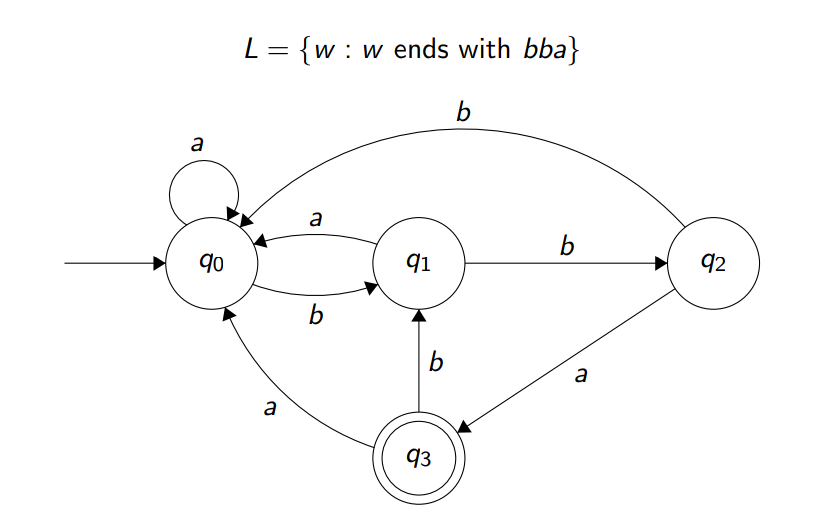
\includegraphics[scale=0.5]{warmup.png}\\
    \item We extend our definition of $\delta : (Q \times \sigma) \rightarrow Q$ to a fn defined over $(Q \times \sigma^*)$ via:
        \begin{align*}
            \delta : (Q \times \sigma^*) &\rightarrow Q \\
            (q, \epsilon) &\mapsto q \\
            (q, aw) &\mapsto \delta^*(\delta(q, a), w) \\
        \end{align*}
    where $a \in \sigma$ and $w \in \sigma^*$.  $aw$ is the concatenation.
\item A DFA given by $M = (\sigma, Q, q_0, A, \delta)$ \textbf{accepts a string} $w$ iff $\delta^*(q_0, w) \in A$.
    \item For example:
        \begin{align*}
            \delta^*(q_0, abba) &= \delta^*(\delta(q_0, a), bba)\\
            &= \delta^*(q_0, bba) \\
            &= \delta^*(q_1, ba) \\
            &= \delta^*(q_2, a) \\
            &= \delta^*(q_3, \epsilon) \\
            &= q_3
        \end{align*}
    \item Essentially, we define $\delta^*$ to be just $\delta$ but now, it supports more than one ``character'', allowing us to traverse the function.
    \item We define \textbf{the language of a DFA}, $M$, to be the set of all strings accepted by $M$, that is, $L(M) = \{w : M \text{ accepts } w\}$.   
    \item \textbf{Kleene's Theorem:} $L$ is regular iff $L = L(M)$ for some DFA $M$.  That is, the regular languages are precisely the languages that are accepted by DFAs.
    \item \textbf{Implementing a DFA:}
        \begin{lstlisting}[mathescape, numbers=none, breaklines=true]
s = $q_0$
while not EOF do
    read character ch
    switch(s)
    case $q_0$:
        switch(ch)
        case ch = $a_0$:
            s = new_state_a_0
        case ch = a_1:
            s = new_state_a_1

        $\cdots$

        case ch = $a_{|\sigma|}$:
            s = new_state_a_sigma
        end switch
    case $q_1$:

        $\cdots$

    end switch
end while
        \end{lstlisting}
    \item Alternatively, we could also use a LUT to store the appropriate states based on $a_x$ and $q_y$.  
    \item We can extend our DFAs to attach actions to arcs.  
    \item For example, consider $L = $ \{binary numbers without leading zeros\}.  We could create a DFA where we also compute the value of the number at the same time, then print the token.
    \item The regular language would be $1(0 | 1)^* 1$.\\
        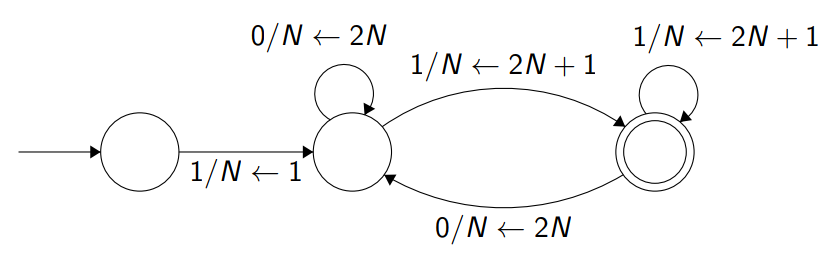
\includegraphics[scale=0.5]{dfa_extend.png}\\
    \item For example, start with 101001:
        \begin{itemize}
            \item 1 $\rightarrow$ N = 1
            \item 10 $\rightarrow$ N = 2
            \item 101 $\rightarrow$ N = 2 * 2 + 1 = 5
            \item 1010 $\rightarrow$ N = 10
            \item 10100 $\rightarrow$ N = 20
            \item 101001 $\rightarrow$ N = 41
        \end{itemize}  
\end{itemize}

\section{Non-deterministic Finite Automata (NFAs)}
\begin{itemize}
    \item What if we are allowed more than one transition from a state?  That is, from, say, $q_0$, I could go to $q_1$ OR $q_2$ based solely on the value of, say, $a$?
    \item When we allow a state to thave multiple branches based on the same input, we say the machine \emph{chooses} what path to go on - this is called \textbf{non-determinism}.
    \item We then say the machine accepts a word $w$ iff there exists \textbf{some} path that leads to an accepting state.
        \newpage
    \item We can simplify our warmup example by using an NFA: \\
        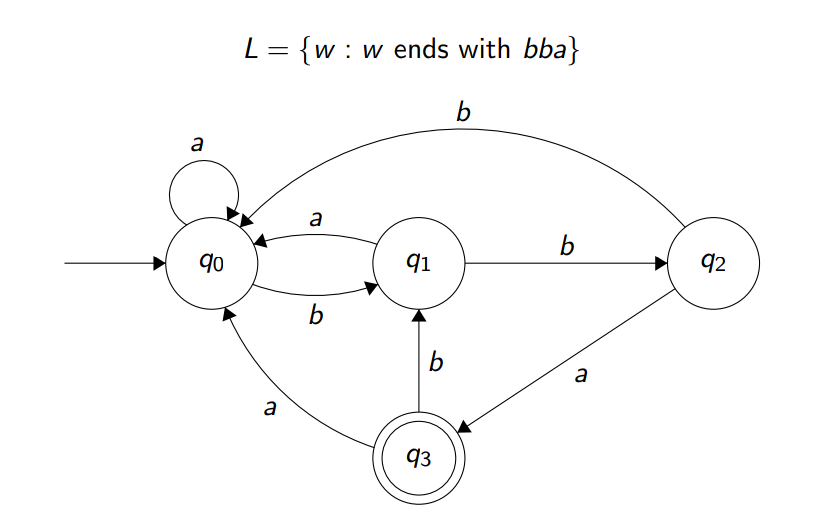
\includegraphics[scale=0.5]{warmup.png}\\
        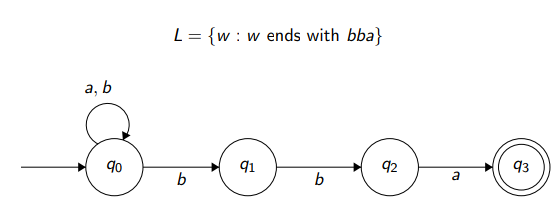
\includegraphics[scale=0.5]{nfawarmup.png}\\
    \item This makes it very easy to extend - if, for example, we wanted to extend this up to z, we can just say that the opening loop goes from a to z.
    \item An \textbf{NFA} is still a 5-tuple.  Nothing changes, except $\delta$.
    \item $\delta$ is now defined as $\delta : (Q \times \sigma) \rightarrow 2^Q$, which is our total transition function.
    \item $2^Q$ denotes the \textbf{power set} of $Q$, that is, the set of all subsets of $Q$.  This allows us to  go to multiple states at once.
    \item For example, if our language is just \{1, 2, 3\}, then $2^Q = \{\{\}, \{1\}, \{2\}, \dots ,\{2, 3\}, \{1, 2, 3\}\}$.
    \item Let $M$ be an NFA.  We say $M$ \textbf{accepts} $w$ iff there exists some path through $M$ that leads to an accepting state.
    \item We denote the \textbf{language of an NFA} $M$ to be the set of all strings accepted by $M$, that is, $L(M) = \{w : M \text{ accepts } w\}$.
    \item We extend $\delta$ for an NFA:
        \begin{align*}
            \delta^* : (2^Q \times \sigma^*) &\rightarrow 2^Q \\
            (S, \epsilon) &\mapsto S \\
            (S, aw) &\mapsto \sigma^* (\bigcup_{q \in S} \sigma(q, a), w) \\
        \end{align*}
            where $a \in \sigma$.  
    \item In other words, an NFA given by $M = (\sigma, Q, q_0, A, \delta)$ \textbf{accepts a string} $w$ iff $\delta^*(\{q_0\}, w) \cap A \not= \varnothing$.
    \item To simulate an NFA:
        \begin{lstlisting}[mathescape, numbers=none, breaklines=true]
S = {$q_0$}
while not EOF do:
    c = read_char()
    S = $\bigcup_{q \in S} \delta(q, c)$
end while
if $S \cap A \not= \varnothing$ then
    Accept
else
    Reject
end if
        \end{lstlisting}
    \item Let us try simulating our warmup example with a NFA:\\
        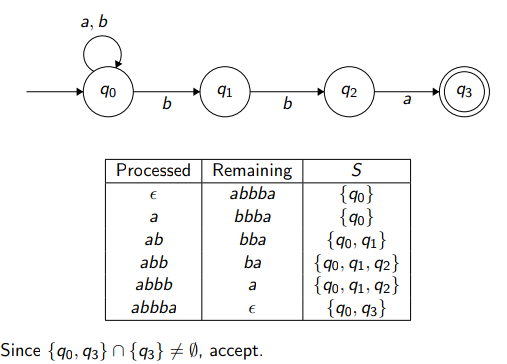
\includegraphics[scale=0.5]{simu.png} \\
\end{itemize}


\end{document}

